\section{Логика работы программы} \label{logic}
\subsection{Структурирование программы по Задачам}
Работа СПО «Кама-Надир» структурирована по решаемым задачам согласно  схеме на Рис.~\ref{fig:general_scheme}.
\begin{figure}[H]
    \centering
    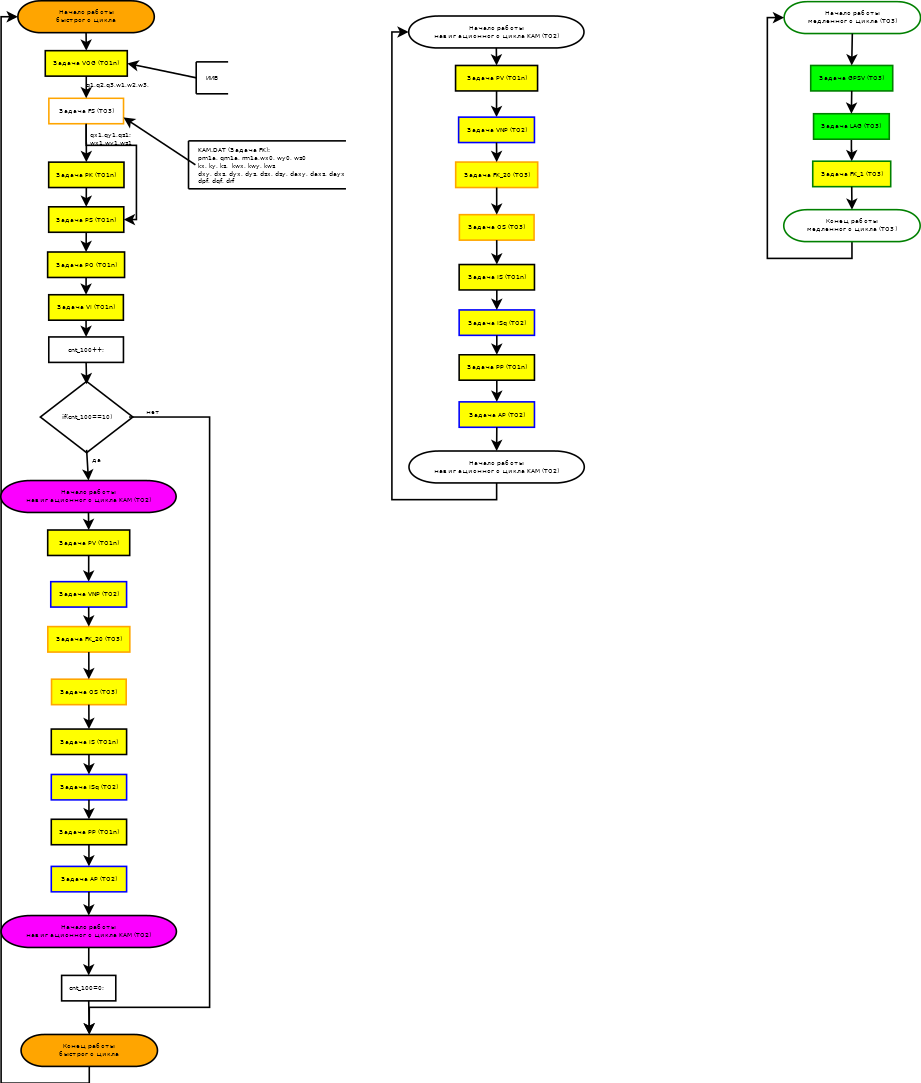
\includegraphics[width=1.0\linewidth]{images/general_scheme.png}
    \caption{Задачи программы}
    \label{fig:general_scheme}
\end{figure}
\subsection{Задача формирования сигналов FS}
Реализует следующие функции согласно схеме на Рис.~\ref{fig:FS}
\begin{figure}[H]
    \centering
    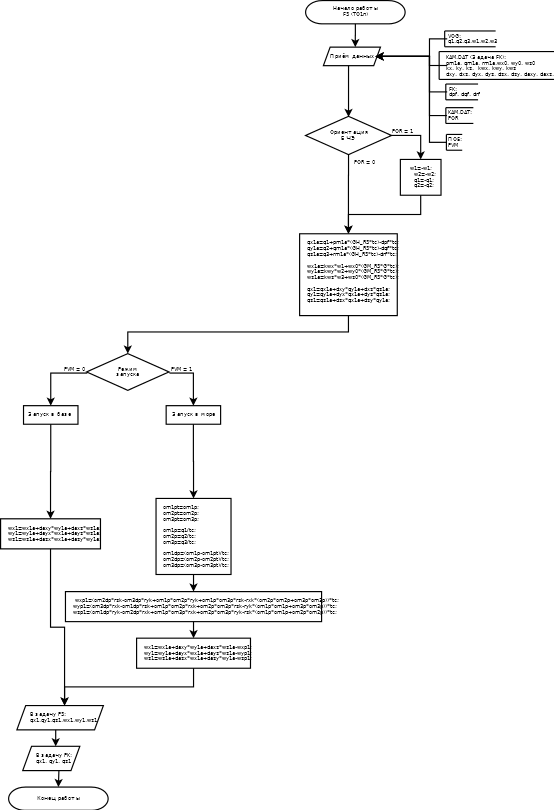
\includegraphics[width=0.8\linewidth]{images/FS.png}
    \caption{Задача FS}
    \label{fig:FS}
\end{figure}
\begin{itemize}
\item Принимает от задачи VOG сигналы - q1,q2,q3,w1,w2,w3 и формирует с учетом принятой модели  инструментальных погрешностей передаваемые в задачи PK и PS  
приращения угла поворота qx1,qy1,qz1 и кажущейся скорости wx1,wy1,wz1 в проекциях на оси БЧЭ.
\item Преобразует сигналы горизонтных каналов ВОГ- q1,q2  к осям обьекта при значении признака ориентации POR=1 в случае установки корпуса БЧЭ 
с поворотом на 180 относительно продольной оси объекта.
\item Осуществляет масштабирование, компенсацию аддитивных и мультипликативных составляющих модели  инструментальных погрешностей   
сигналов ВОГ и акселерометров с использованием задаваемых в случае необходимости в файле данных KAM.DAT корректур, а также меняющихся в запуске 
и  оцениваемых оптимальным фильтром Калмана ( ОФК ) составляющих дрейфов в осях БЧЭ:  
    \begin{itemize}
\item систематических ошибок  pm1a, qm1a, rm1a,wx0, wy0, wz0
\item масштабных коэффициентов kx, ky, kz,  kwx, kwy, kwz
\item невыставок  dxy, dxz, dyx, dyz, dzx, dzy, dаxy, dаxz, dаyx
\item оценки дрейфов dpf, dqf, drf
    \end{itemize}
\end{itemize}
\subsubsection{Входные и выходные данные задачи FS}
Входная информация
\begin{itemize}
    \item q1, q2, q3, w1,w2,w3- из задачи  VOG-приема сигналов БЧЭ
    \item pm1a,qm1a, rm1a, wx0, wy0, wz0, kwx, kwy, kwz, dxy, dxz, dyx, dyz, dzx, dzy, daxy, daxz, dayx, dayz, dazx, dazy - из файла данных kam.dat
    \item dpf, dqf, drf- из задачи  FK
\end{itemize}
Выходная информация
\begin{itemize}
    \item qx1, qy1, qz1- в задачу PK
    \item qx1,qy1,qz1,wx1,wy1,wz1-- в задачу PS
\end{itemize}
